\chapter{Desarrollo}
\label{cap:Desarrollo}

\setlength{\parindent}{0pt}

En este capítulo se hablará del desarrollo de la aplicación Android (diseño, funcionalidades\dots) que he estado realizando a lo largo del TFG, así como el registro de claves para poder interacturar con la red blockchain que se ha levantado. También, se explicará en que consiste el SDK desarrollado, cuales son sus funcionalidades y como poder utilizarlo para otras aplicaciones Android.

% ##################################################
% ##################################################
\section{Aplicación Android}

Para el desarrollo de la aplicación móvil, se ha decidido enfocarlo únicamente a aplicaciones Android. Lógicamente, en un futuro, se tendrá que adapatar una aplicación para otros sistemas como iOS. O por el contrario reescribir él código con lenguajes ````cross platform'' para permitir el correcto funcionamiento nativo tanto en Android como en iOS, una buena opción es utilizar \textbf{flutter}\cite{flutter}.

% --------------------------------------------------
\subsection{Conceptos Básicos de Android}

A la hora de programar aplicaciones en Android, lo ideal es trabajar en paralelo con la documentación para desarrolladores\cite{androidDocs}. En ella se detalla el completo funcionamiento y diferentes APIs disponibles para programar las aplicaciones. Para este apartado resumo algunos de los conceptos de la guia, siendo una gran recomendación si se quiere profundizar más ir direcamente a la guia. \\

Las aplicaciones de Android se pueden escribir con \textbf{Kotlin, Java y C++}\cite{kotlin,java,c++}. Una vez escrito el código fuente, las herramientas de Android SDK compilan el código generando un paquete o APK, el cual incluye todos los contenidos de la aplicación Android y permite ser ejecutado en un dispositivo móvil (el dispositivo requerirá de la versión Android mínima para poder ejecutar.). \\

Cada aplicación de Android resite en su propia ``zona virtual'', un conjunto de factores permiten tener aisladas las aplicaciones Android del resto del móvil. Entre otras, puesto que Android reside en un sistema Linux, el cual es multiusuario, cada aplicación en el móvil es un usuario el cual puede acceder solo a sus archivos y documentos teniendo sus propios permisos como usuario dentro del dispositivo y creando lo grupos que necesite. Cada proceso que se ejecuta tiene su propia máquina virtual, ejecutandose el código de forma independiente al reso de aplicaciones. Es el sistema operativo el que se encarga de mantener los distintos procesos, así como arrancar procesos que sean requeridos por la aplicación. \\

Un ejemplo, si desde la aplicación de galeria queremos compartir una foto por whatsapp, la aplicación ``galeria'' le pedirá al SO que ejecute una actividad de ``whatsapp'' y será el SO quien se encarge de decidir si tiene permiso para eso o no, o si tiene recursos para ejecutarlo o no. En ningún momento la aplicación ``galeria'' tiene libertad para ejecutar otros procesos. \\

De forma predeterminada las aplicaciones solo tiene derecho de usar sus propios archivos, pero puede pedir permiso al sistema operativo para guardar información en el dispositivo, en el caso de mi aplicación Android por ejemplo, el registro de claves para acceder a la blockchain se guardan de forma local en el dispositivo. También, la aplicaciones pueden pedir permiso para utilizar cámara, conexión bluetooth\dots \\

Por úlimo, algo muy importante a tener en cuenta al programar aplicaciones Android es que no puedes hacer operaciones pesadas en el hilo de ejecución principal. Todas las ejecuciones pesadas deben hacerse en otro hilo y con un callback recuperar la información si es necesario. Por ejemplo, al hacer llamdas a una API estas llamdas deben hacerse en otro hilo de ejecución diferente. Android no permite que bloquees la interfaz de usuario con operaciones pesadas (como una llamada a una API).

\subsubsection{Componentes de la aplicación}

Las aplicaciones Android tienen:
\begin{itemize}
    \item Actividades
    \item Servicios
    \item Receptores de emisiones
    \item Proveedores de contenido
\end{itemize}
\vspace{0.5cm}
\textbf{Actividades} \\
Las \textbf{Actividades} son el punto de entrada de interacción con el usuario. Se representan como una pantalla con una interfaz de usuario. Por ejemplo, whatsapp tiene una actividad que es la pantalla en la que todos los grupos y gente con la que hablas, y al entrar en un grupo, whatsapp ejecuta una actividad diferente. Las actividades trabajan juntas pero son independientes entre si, brindando la posibilidad de llamar a una actividad concreta desde otra aplicación. Si quieres compartir una foto con un grupo en whatsapp, desde la app de galeria seleccionas la foto y llamas a la actividad de whatsapp del grupo de amigos concreto con quienes quieres compartir la foto. Las actividades permiten:

\begin{itemize}
\item Realizar un seguimiento de la pantalla que esta viendo el usuario.
\item Permitir regresar a actividades anteriores (actividades detenidas) a las que puede volver el usuario si lo desea, priorizando entonces algunos procesos mas que otros.
\item Permitir finalizar procesos, volviendo a la actividad anterior.
\item Permitir ser llamadas desde otras aplicaciones (como el ejemplo de compartir una imagen)
\end{itemize}

\vspace{0.5cm}
\textbf{Servicios} \\
Los \textbf{Servicios} son un punto de entrada general que permite mantener en ejecución una aplicación en segundo plano y no proporcionan una interfaz de usuario. Un servicio puede reproducir música, sincronizar datos\dots Además los servicios pueden dividirse en 2, \textbf{servicios iniciados} y \textbf{servicios enlazados}. Los iniciados son servicios que inicia el usuario como reproducir música dejando luego el proceso en segundo plano. Y un servicio enlazado sería cuando una aplicación hace uso de otra para alguna tarea. Esta segunda aplicación que esta siendo usada, se ejecuta en segundo plano como servicio enlazado. \\

\textbf{Receptores de emisiones} \\
Los \textbf{receptores} permiten que el sistema entregue eventos a una aplicación fuera del flujo habitual. El sistema puede entregar emisión de aplicaciones que no estan en ejecución. Por ejemplo, una aplicación programa una alarma a una hora determinada, aunque la aplicación no este en ejecución, la alarma sonará a la hora establecida. Muchas de las emisiones, vienen del propio sistema. Por ejemplo, pantalla apagada, batería baja, captura de pantalla\dots Los receptores de emision no disponen de interfaz de usuario, pero a traves de la API de Android pueden mostrar mensajes en la barra de tareas. \\

\textbf{Proveedores de contenido} \\
Los \textbf{proveedores de contenido} administran conjuntos compartidos de datos de la aplicación que pueden ser almacenados en el sistema de archivos, en una BDD o en la web. A traves del proveedor de contenido, otras aplicaciones pueden acceder a esos datos (siempre que tengan permiso). Por ejemplo, la aplicación de contactos del móvil, tiene un proveedor de contenido, lo que permite a otras aplicaciones pedir acceso a la agenda de datos (siendo el usuario el que acepta que la aplicación acceda a los contactos). También son útiles para leer y escribir datos privados que no quieras compartir con otras aplicaciones.

\subsubsection{Activación de componentes}

Un aspecto exclusivo de Android es que cualquier aplicación puede iniciar un componente de otra aplicación. Si quieres que el usuario tome una foto, no hace falta desarrollar la comunicación con el hardware de la camara, sino que simplemente puedes llamar a la aplicación de la camara la cual te devolverá la foto que el usuario tome. Por ejemplo, si inicias la actividad de la camara, la actividad se ejecuta en el proceso de la camara no en tú aplicación. Por lo tanto, a diferencia de lo que sucede en las aplicaciones de otros sitemas, aquí no existe un método principal o \verb|main()|. Android no tiene un único punto de entrada. \\

De los cuatro tipos de componente, actividades, servicios y receptores se activan mediante un mensaje asíncrono denominado \verb |intent|, estos vinculan componentes entre sí durante el tiempo de ejecución. Son algo así como mensajeros. Sin embargo, los proveedores de contenido se activan con solicitudes de un \verb|ContentResolver|. Además, existen para cada componente métodos independientes para activarlos según el objetivo que se busque.
\subsubsection{El archivo de manifiesto}

Para que Android pueda iniciar un componente, debe reconocer la existencia de ese componente leyendo el archivo de manifiesto de la aplicación, \verb|AndroidManifest.xml|. El manifiesto puede hacer lo siguiente:
\begin{enumerate}
    \item Declarar los componentes de la aplicación
    \item Identificar los permisos de usuario que requiere la aplicación (acceso a internet, o acceso a los contactos)
    \item Declarar caracterisiticas hardware y software así como nivel de API mínimo.
    \item Declarar APIs a las que la aplicación necesita estar vinculado (como la biblioteca de google maps)
\end{enumerate}

\subsubsection{Recursos de la aplicación}

Las aplicaciones Android se componen de mucho más que solo código. Disponen de imágener, vídeos, fuentes, audios y otros elementos como las interfaces de usuario en XML. Los recursos facilitan la actualización de las características de la aplicación para permitir el cambio de idioma, de fuente, de tamaño según el dispositivo\dots \\

Por cada recurso, el SDK define un ID con número entero único para poder hacerle referencia. Estos IDs se utilizan en el código, por ejemplo, para añadir una imágen puedes hacer referencia al ID de la imágen asignado por el SDK. Una de las ventajas de utilizar los recursos, es facilitar la traducción de la aplicación a otros idiomas, también puedes mostrar parte de la interfaz de usuario si el usuario tiene una suscripción concreta u otra. En el caso de mi aplicación móvil, utilizo esto para mostrar una aplicación diferente  a los alumnos y profesores.

\clearpage
% --------------------------------------------------
\subsection{Diseño de la Aplicación}

A la hora de pensar en el diseño completo del proyecto, decidí utilizar un diseño modular soportado por APIs, esto me permite tener múltiples componentes independientes los cuales trabajan juntos. Gracias a esto, cambios en el código de un componente o API, son completamente transparentes para el resto de APIs. El proyecto dispone entonces de 3 APIs. Tenemos, la API que se comunica con la base de datos, la API que se comunica con la red blockchain, y la API que hace de intermediario para que el móvil no tenga que comunicarse con las otras dos APIs centrando así la comunicación. Además, el dispositivo móvil se comunica también con la red blockchain para algunas tareas que expongo en la seccion \hyperref[sec:SDK]{SDK}. De estos componentes los que nos interesan para este trabajo son la aplicación Android y la API de microservicios, ambos desarrollados a lo largo del trabajo de fin de grado, la API de la base de datos y la red blockchain fueron desarrolladas con anterioridad al TFG. 

\subsubsection{Arquitectura}
\begin{figure}[h!]
  \centering
  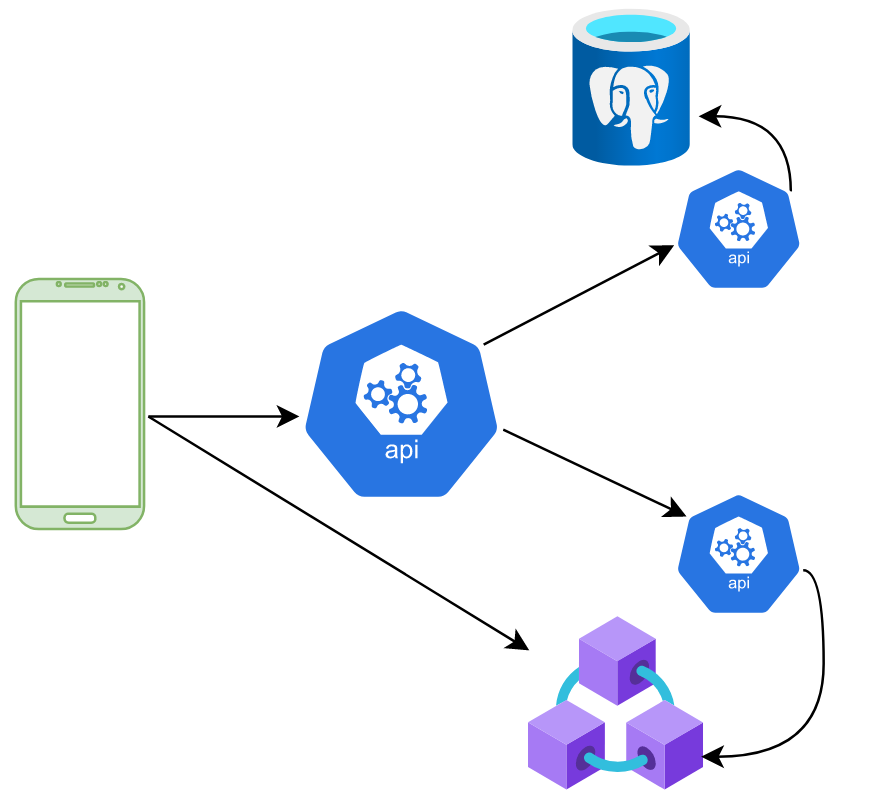
\includegraphics[width=0.6\linewidth]{figs/Desarrollo/Arquitectura}
  \caption[Arquitectura]{Arquitectura Completa del proyecto}
  \label{fig:estublockArch}
\end{figure}

El dispositivo móvil se comunica con la api de microservicios a través de dos librerias que veremos más en profundidad en \hyperref[sec:Codigo]{Codigo} esta a su vez se comunica con la API de la base de datos o de la red blockchain según la operación que se haya especificado y estas se comunican con el servidor postgresql para la base de datos y la red de quorum para la blockchain. Como pequeño apartado, la API que se comunica con el servidor postgresql esta desarrollada con NodeJS y utiliza la librería \emph{node-postgres} y la API que se comunica con quorum también esta desarrollada con NodeJS y utiliza la libreria \emph{web3} para comunicarse con la red blockchain. 

% --------------------------------------------------
\subsection{Desarrollo de Microservicio Externo}

El objetivo de desarrollar una API extra con la que centralizar las llamadas a la base de datos y a la red blockchain, es para agilizar las llamadas y tratamiento de datos por parte del dispositivo móvil, así como minimizar la cantidad de código, tamaño de la apliación móvil, dependencias del proyecto\dots La API de microservicios con la que se comunica la aplicación móvil esta desarrollada utilizando \textbf{NodeJS} y ha sido documentada utilizando \textbf{Swagger} como se puede ver en la siguiente imágen.

\begin{figure}[hbt]
	\centering
	\begin{subfigure}[b]{0.4\linewidth}
		\centering
        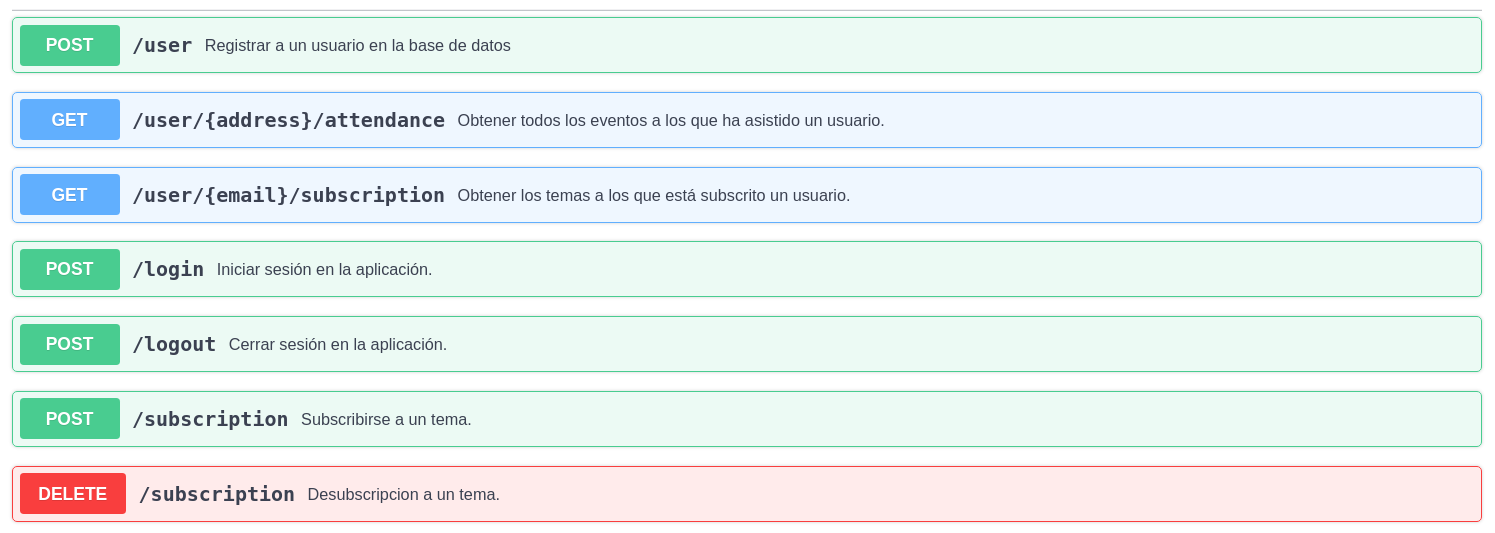
\includegraphics[width=0.6\linewidth]{figs/Desarrollo/Swagger}
        \caption[Swagger]{Fragmento de documentación en Swagger del Proyecto}
	\end{subfigure} 
	\begin{subfigure}[b]{0.4\linewidth}
		\centering
        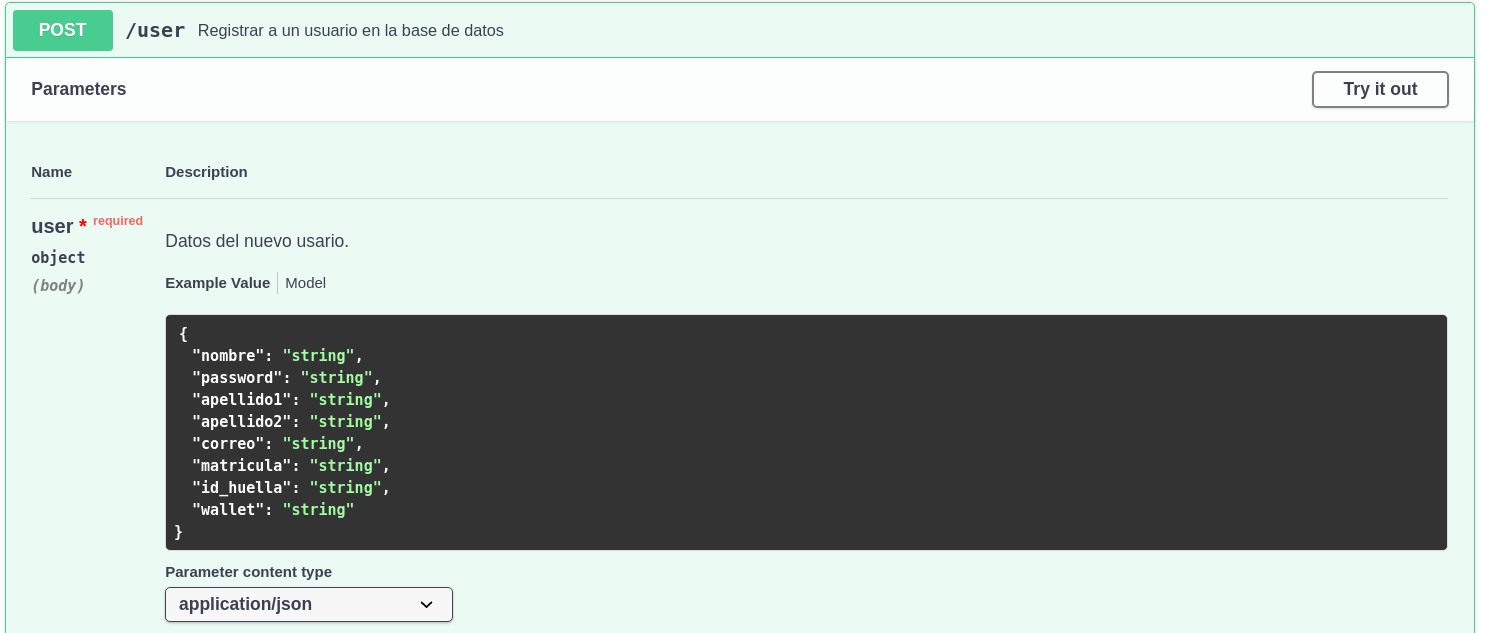
\includegraphics[width=0.6\linewidth]{figs/Desarrollo/SwaggerUsuario}
        \caption[Swagger Usuario]{Fragmento de documentación de crear usuario}
	\end{subfigure} 
	\caption[Swagger]{Documentación con Swagger}
	\label{fig:programas}
\end{figure}

% --------------------------------------------------
\subsubsection{NodeJS}
Node.js\cite{nodejs} es un entorno de ejecución de \textbf{JavaScript} contruido con el motor de \emph{JavaScript V8 de Chrome}. Esta ideado como un entorno orientado a eventos asíncronos con el que se pueden diseñar aplicaciones escalables en la red. Permite tratar múltiples conexiones simultaneas sin que el programador tenga que preocuparse por la concurrencia. Hoy en día, los modelos de concurrencia usan hilos del sistema operativo y requieren de bloquear procesos para operaciones de lectura y escritura. Los usuarios de NodeJS están libres de preocuparse por el bloqueo del proceso, ya que no existe. De ahí que sea muy propicio desarrollar sistemas escalables con NodeJS, de todos modos aunque NodeJS trabaja sin hilos, se pueden aprovechar múltiples núcleos en su entorno, generando varios procesos. \\

He decidido utilizar NodeJS para desarrollar la API de microservicios pues me da la seguridad de que responderá correctamente a miles de llamadas simultaneas (siempre y cuando el servidor en el que se este ejecutando pueda con el poder de computo que ello requiere). Así pues, puedo estar tranquilo y saber que el sistema no se caerá y podrá dar servicio un largo tiempo. Además, NodeJS junto con su gestor de paquetes \emph{npm} me permiten mantener el sistema actualizado con facilidad sin preocuparme de problemas de dependencias y paquetes desactualizados o que tienen problemas de seguridad. \\

Algunos ejemplos de grandes proyectos que utilizan NodeJS son:
\begin{itemize}
\item Netflix
\item Trello
\item PayPal
\item LinkedIn
\item Uber
\end{itemize}

% --------------------------------------------------
\subsubsection{Swagger}
A la hora de programar una API, no es solo importante que el código sea correcto y funcione correcta y eficientemente. Sino que también es muy importante la documentación de la API, esto permite a otros programadores poder utilizarla sin preocuparse del código, y sin necesidad de conocer el proyecto. Para ello, he utilizado \textbf{Swagger} \cite{swagger}. Swagger es un conjuneto de herramientas profesionales y de código abierto las cuales ayudan a diseñar y documentar APIs de forma escalable. Swagger permite hacer varias cosas:
\begin{itemize}
\item Diseñar
\item Desarrollar
\item Documentar
\item Testear
\item Virtualizar
\item Monitorizar
\end{itemize}

Para este proyecto, me aproveche principalmente de las herramientas de diseño, desarrollo y documentación. Centrandome sobre todo en la comodidad de documentación que tiene al utilizar archivos \emph{YAML} (yaml es un formato de serialización de datos legibles por humanos) para generar una docuementación ligera, fácil de entender y muy detallada. 

% --------------------------------------------------
\subsubsection{Funcionalidades de la API de Microservicios}
Las funcionalidades de la API se pueden dividir en los siguientes 3 casos de uso generales:

\begin{figure}[h!]
  \centering
  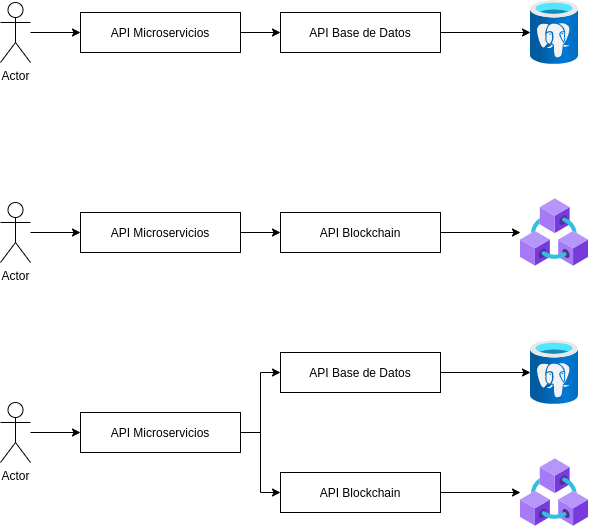
\includegraphics[width=0.6\linewidth]{figs/Desarrollo/UML}
  \caption[Arquitectura]{Los tres casos de uso general de la aplicación}
  \label{fig:casosUso}
\end{figure}

Siendo más concretos pasemos a listar todas las funcionalidades de las que dispone la API, lógicamente esta no es la documentación completa la cual trae consigo los objetos JSON que aceptan la URIs y los errores u objetos JSON que devuelve cada una de las URIs. En el presente la documentación se mantiene en un repositorio de \emph{gitlab} privado. \\

\begin{itemize}
\item \textcolor{green}{{\footnotesize POST} /user:} Permite registrar a un usuario en la base de datos.
\item \textcolor{blue}{{\footnotesize GET} /user/{address}/attendance:} Permite obtener los eventos a los que ha asistido un usuario.
\item \textcolor{blue}{{\footnotesize GET} /user/{email}/subscription:} Permite obtener los temas a los que está suscrito un usuario.
\item \textcolor{green}{{\footnotesize POST} /login:} Permite iniciar sesion (se comprueba que el usuario exista y se comprueba la contraseña hasheada).
\item \textcolor{green}{{\footnotesize POST} /logout:} Permite detectar que un usuario ha cerrado sesion.
\item \textcolor{green}{{\footnotesize POST} /subscription:} Permite a un usuario suscribirse a un tema.
\item \textcolor{red}{{\footnotesize DELETE} /subscription:} Permite a un usuario desuscribirse de un tema.
\item \textcolor{blue}{{\footnotesize GET} /topic:} Permite obtener la lista de temas disponibles.
\item \textcolor{blue}{{\footnotesize GET} /topic/{id}/event:} Permite obtener un listado de los eventos de un tema concreto.
\item \textcolor{blue}{{\footnotesize GET} /topic/{id}/subscription:} Permite obetner un listado con las suscripciones de un tema.
\item \textcolor{green}{{\footnotesize POST} /event:} Permite obtener los datos de la transaccion de crear un evento, esta es firmada por el usuario a través de la aplicación Móvil y despues enviada a la red blockchain. 
\item \textcolor{blue}{{\footnotesize GET} /event/{id}:} Permite obtener los datos de un evento.
\item \textcolor{orange}{{\footnotesize PUT} /event/{id}:} Permite obtener los datos de la transaccion para modificar un evento, también se firma y envia desde el móvil a la red blockchain. 
\item \textcolor{blue}{{\footnotesize GET} /event/{id}/delete/{organizer}:} Permite obtener los parámetros de la transaccion para cerrar un evento, se firma y envia desde el móvil.
\item \textcolor{blue}{{\footnotesize GET} /eventCatalog:} Permite obtiene un listado con los tipos de eventos. 
\item \textcolor{green}{{\footnotesize POST} /event/{id}/validator:} Permite añadir a un nuevo validador a un evento.
\item \textcolor{blue}{{\footnotesize GET} /event/{id}/validator/{organizer}:} Permite obtener un listado con los validadores de un evento. 
\item \textcolor{orange}{{\footnotesize POST} /event/{id}/attendance:} Permite obtener los parámetros de la transaccion para registrar la asistencia a un evento, igual que antes, se firma y envia desde el móvil. 
\item \textcolor{blue}{{\footnotesize GET} /event/{id}/attendance:} Permite obtener la lista de asistencias a un evento. 
\end{itemize}

Gracias a usar swagger, la API sigue la documentación de forma estricta, es decir, no acepta llamadas en las que no se envien los parámetro especificados en la documentación. Si para crear un usuario se requiere de un campo ``email'', si este campo no existe al hacer la llamada a la API, swagger se encarga de rechazar la llamada con un error de formato. Así logramos evitar que el backend tenga errores por variables indefinidas, nulas, o se guarden datos vacíos\dots

% --------------------------------------------------
\subsection{Interaz de Usuario}

La interfaz de usuario es donde los usuarios interaccionan con tu aplicación. Son las ventanas, botones, pantallas con las que el usuario interacciona. Deben tener un diseño intuitivo, fácil, que brinde una experiencia positiva. A más fácil de entender, mejor. Existen tres grandes tipos de interfaces de usuario, la interfaz de lenguaje natural, es la ideal y el sueño de todo usuario, pues permite comunicar humano y máquina con lenguaje natural. Un ejemplo de dispositivo que utiliza esta interfaz es \emph{Alexa}, que cuenta con un software basado en modelos acústicos y del lenguaje. El segundo tipo de interfaz es la interfaz de preguntas y respuestas. En esta interfaz se muestra una pregunta al usuario y según su respuesta se actua de una u otra manera. Un ejemplo de estas interfacez son los software de instalación, como puede ser el instalador de un sistema operativo. Y por último, la interfaz que más nos interesa para este proyecto, la \textbf{interfaz gráfica de usuario}, en inglés ``Graphical User Interface'' o \textbf{GUI}. Esta utiliza gráficos, imágenes, videos, icónos, menús\dots para permitir al usuario interaccionar con la aplicación. 

\subsubsection{Diseño de la GUI de Estublock}

A la hora de diseñar la aplicación Estublock, he buscado un diseño ligero, intuitivo y rápido. Como tiene que llegar a muchos usuarios, hay que pensar en posibles problemas de visión, daltonismo, evitar que se pueda mal interpretar un botón, y que el usuario crea que hace una cosa que no hace. Para todo ello, he utilizado una herramienta de diseño para prototipado de pantallas y testeo de pantallas llamado \emph{Marvel}\cite{marvelapp}. Marvel te permite diseñar con bastante detalle aplicaciones móvil y web, y además permite enlazar pantallas para probar la efectividad de las pantallas y el entendimiento de las mismas.

\subsubsection{Interfaces en Android}

En android la interfaz de usuario se contruye mediante una jerarquía de objetos, generalmente de tipo \textbf{View y ViewGroup}. Los \emph{View} son componentes con los que el usuario puede interactuar, el usuario puede ver el componente en la pantalla. Sin embargo los \emph{ViewGroup} son un contenedor invisible que define la estructura de objetos \emph{View} y otros \emph{ViewGroup}.

\begin{figure}[h!]
  \centering
  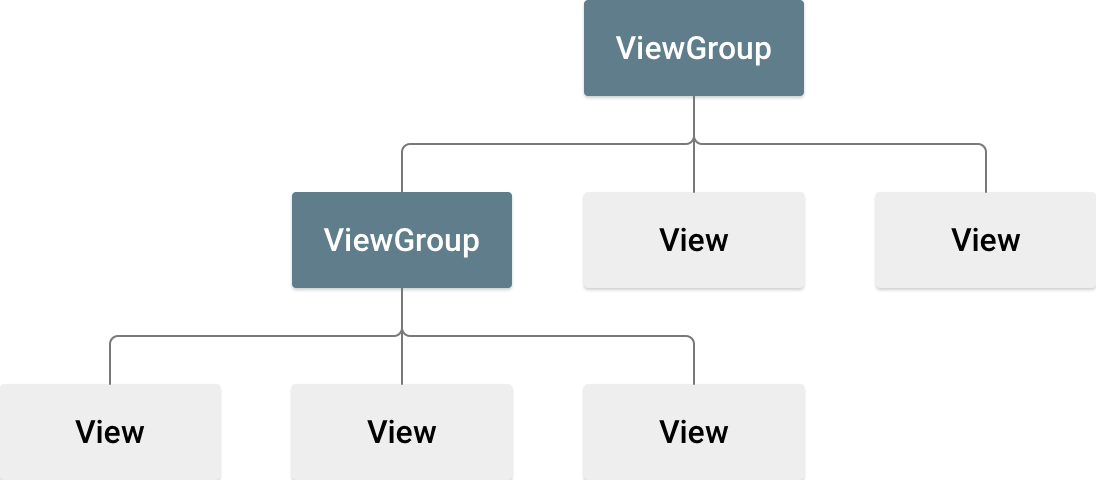
\includegraphics[width=0.6\linewidth]{figs/Desarrollo/Jerarquia}
  \caption[Android Layout]{Jerarquia de una interfaz de Android}
  \label{fig:interfaz_android}
\end{figure}

Los objetos \emph{View} se denominan ``widgets'' y pueden ser Botones, Textos, ``Switch'', ``ScrollView''\dots. Los objetos \emph{ViewGroup} se denominan ``diseño'' y pueden ser ``LinearLayout'', ``ConstraintLayout''\dots Los diseños se pueden declarar de dos maneras: \\

\begin{itemize}
\item Se pueden declarar elementos de la Interfaz de Usuario en \textbf{XML}
\item Crear una instancia de elementos de diseño durante el tiempo de ejecución.
\end{itemize}

Para la aplicación, he usado ambas formas, pues por un lado hay pantallas estáticas, como pueden ser la pantalla de login o registro. En las que se que botónes tiene que haber, que textos tiene que mostrar y que diseño tiene. Pero también hay pantallas en las que se crean botones o texto de forma dinámica dependiendo de el número de temas que haya en la base de datos o según a que temas este suscrita una persona. \\

Gracias a utilizar los archivos XML, puedes separar la presentación de la app del código que controla los componentes, además, facilita la creación de distintos diseños para diferentes tamaños de pantalla y orientación. Es la mejor opción a la hora de crear una GUI aunque en ocasiones se requiera de hacer en tiempo de ejecución. También se puede crear con XML un diseño, y luego modificarlo en tiempo de ejecución según sea necesario. 

% --------------------------------------------------
\subsection{Codigo} \label{sec:Codigo}

Las aplicaciones Android pueden ser programadas principalmente en dos lenguajes de programación, \textbf{Java} y \textbf{Kotlin}. En el presente, la inmensa mayoría de aplicaciones han sido desarrolladas con Java, sin embargo Kotlin es el futuro, en el presente sigue siendo un lenguaje secundario (aunque se puede hacer todo lo que se puede hacer con Java y esta muy bien documentado) de hecho según google trends, Kotlin esta lejos de quitarle el puesto a Java aunque los nuevos desarrolladores de aplicaciones Android muestran más interés por Kotlin por su comodidad, falta de verbosidad y ``limpieza'' (es decir, con menos líneas de código haces lo mismo que Java). 

\begin{figure}[h!]
  \centering
  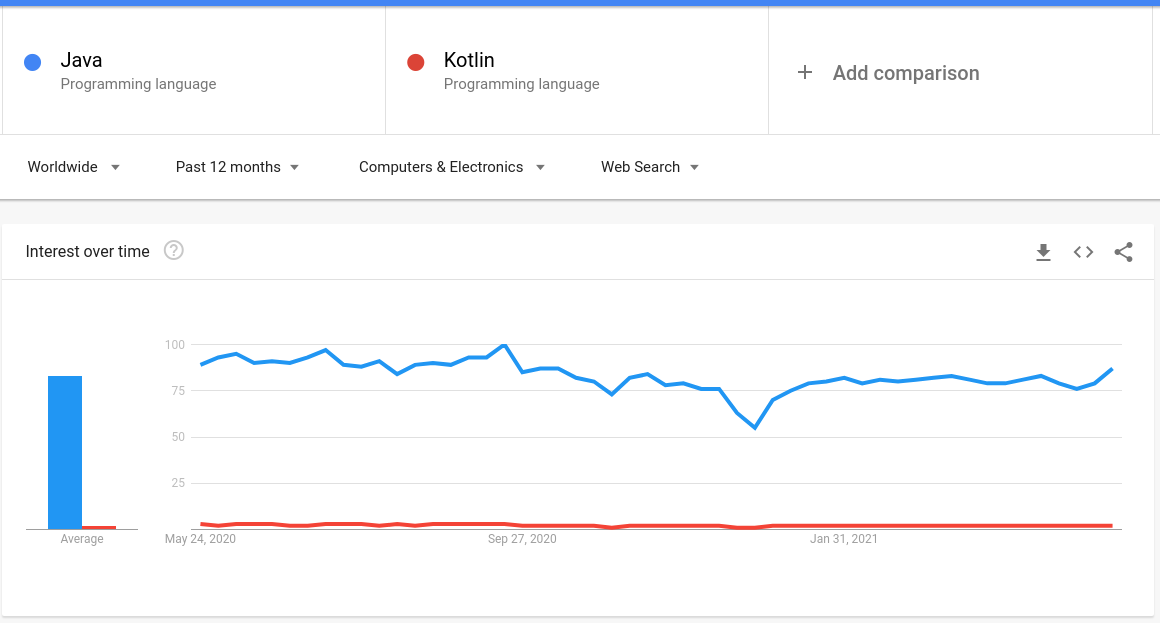
\includegraphics[width=0.6\linewidth]{figs/Desarrollo/Popularidad}
  \caption[Java vs Kotlin]{Comparación de Google Trends entre Java y kotlin}
  \label{fig:java_vs_kotlin}
\end{figure}

Por lo tanto, aunque Kotlin promete mucho, he desarrollado la aplicación Estublock en Java. Por suerte, se puede migrar con múcha facilidad a Kotlin puesto que AndroidStudio (el Entodno de Desarrollo Integrado para programar aplicaciones Android) permite migrar automáticamente de Java a Kotlin. Para facilitar este proceso se deben poner ``marcas'' que especifiquen las caracteristicas de algunas variables o funciones para facilitar a AndroidStudio el reconocimiento de las variables. Un ejemplo puede encontrarse a continuación donde se puede ver que se especifica que las variables no pueden ser nulas con \emph{@NonNull}.

\begin{lstlisting}[language=Java,float=ht,caption={[Java] Ejemplo de ``etiquetado'' de variables para facilitar el salto a Kotlin},label=lst:java_etiquetas]
public void sendSignedTransaction(@NonNull String signedMessage){
  // Código
}
\end{lstlisting}

% --------------------------------------------------
\subsubsection{Codigo XML}

Como ya hemos mencionado, las interfaces de usuario en Android se programan utilizando archivos XML. XML del ingles \emph{Extensible Markup Language} es un metalenguaje que permite definir un lenguaje de marcas el cual es utilizado para almacenar datos de forma legible. Permite crear estructuras con parámetros y atributos. A la hora de programar en Android Studio con XML se tienen dos opciones, se puede escribir directamente el código XML o se pude utilizar la herramienta que viene integrada en AndroidStudio con la que se pueden crear elementos y añadirles atributos sin necesidad de programar directamente el XML. 

\begin{figure}[h!]
  \centering
  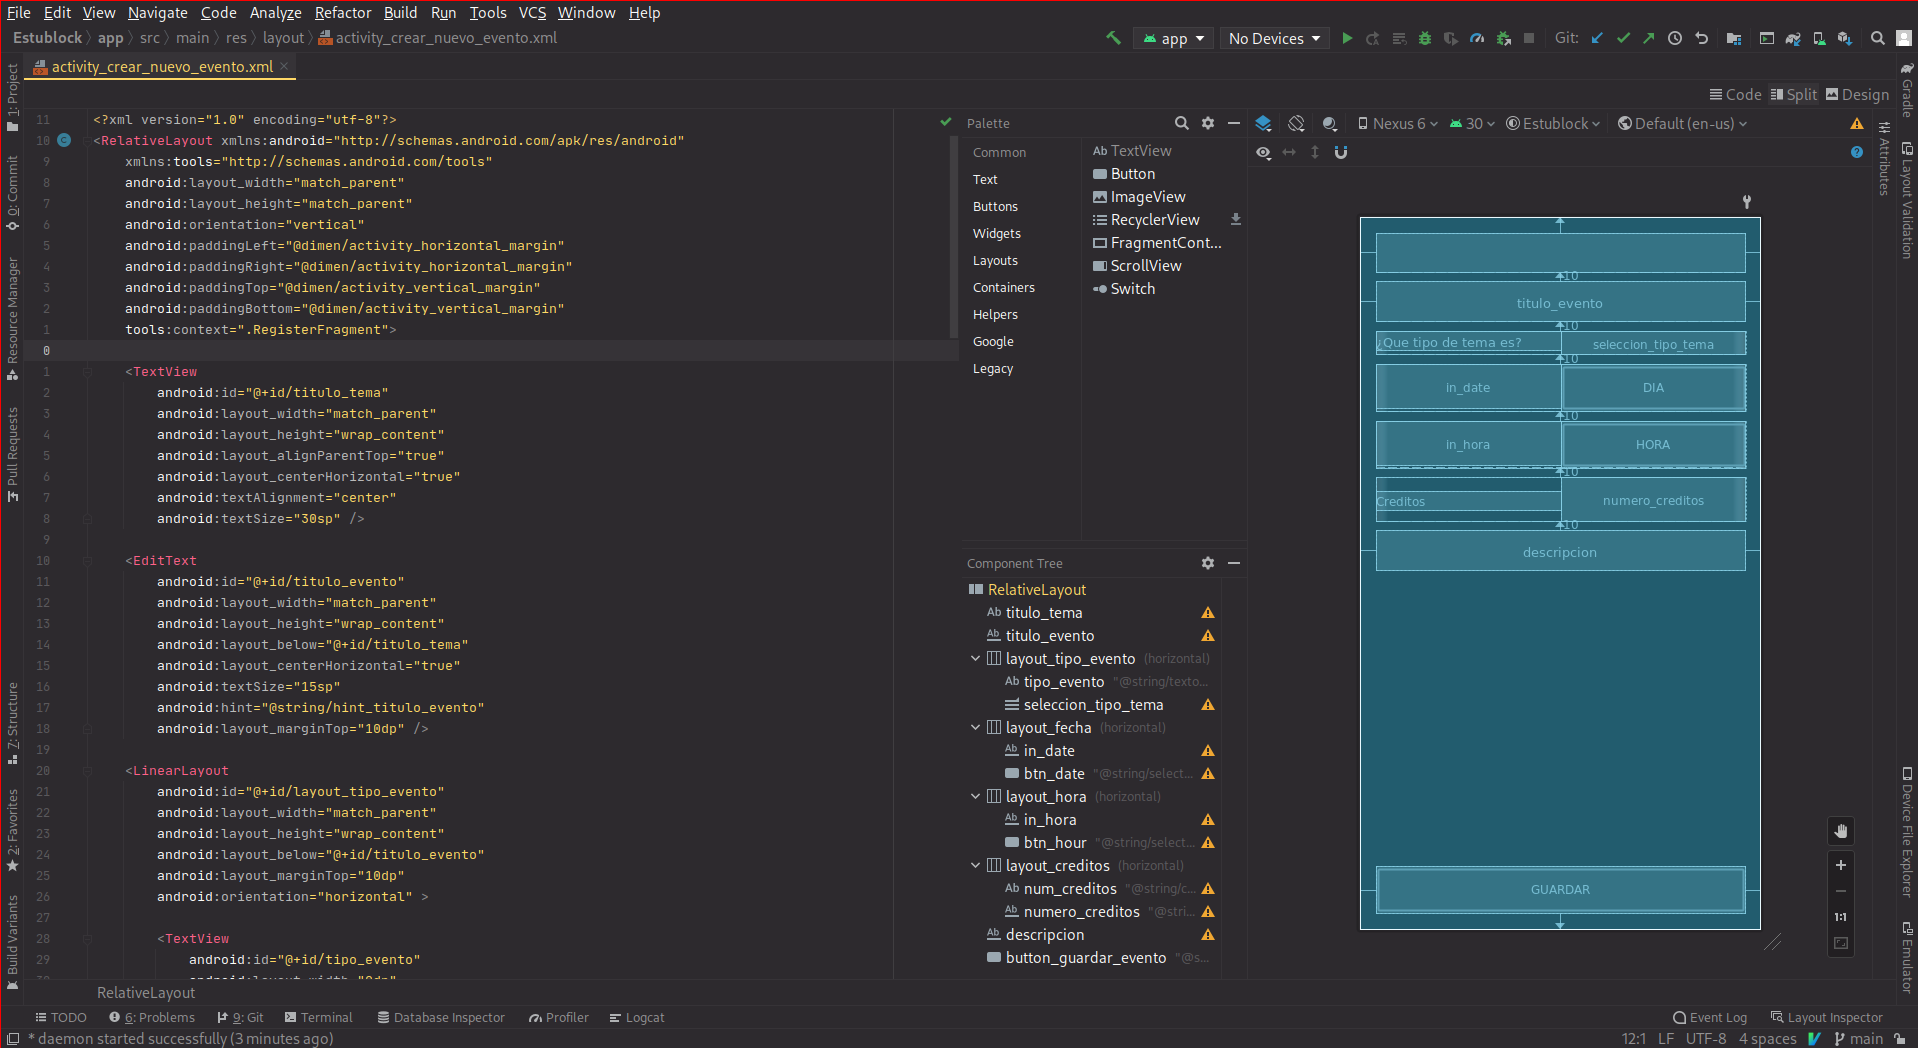
\includegraphics[width=0.95\linewidth]{figs/Desarrollo/xml_vs_ezpz}
  \caption[XML]{Codigo XML y su correspondiente en la herramienta de AndroidStudio}
  \label{fig:xml_vs_ezpz}
\end{figure}

Aunque la herramienta de AndroidStudio es muy útil, la mayoría de las pantallas han sido programadas editando el código XML directamente y viendo el resultado en la herramieta de AndroidStudio.

% --------------------------------------------------
\subsubsection{Codigo Java}

Todo el código de la aplicación esta disonible en mi repositorio de github\cite{forgis98}. Vamos a tratar de resumir el trabajo realizado, pues gran parte de este TFG esta reflejado en la aplicación móvil que se ha desarrollado. \\

\myuline{Archivos del Proyecto} \\

El proyecto puede dividirse en 2, el SDK del que hablaremos más adelante. En él esta el código que se comunica con la red blockchain. Y por otro lado estan las actividades y fragmentos que se comunican con sus respectivas pantallas, a excepción de un archivo llamando \meph{GlobalState.java}. Este archivo es muy importante, pues sirve para mantener el estado en tiempo de ejecución del proyecto. Guarda información como el nombre de la persona una vez ha hecho login, guarda él directorio de la cartera virtual del usuario, contiene la URL a las APIs de microservicios, red blockchain y demás datos necesarios. \\

A parte de esto, hay una carpeta más, llamada \emph{preferences o shared preferences}. Android proporciona muchas formas de almacenar los datos de una aplicación, y esta es una de ellas. Las preferencias permiten guardar datos en forma de un par \{claves $->$ valor\}. Utilizo este archivo para guardar el correo del usuario asociado con la dirección en la que esta su cartera virtual. Esto permite al usuario tener varias cuentas en el móvil sin que haya conflicto entre las carteras virtuales. 

\myuline{Librerias utilizadas} \\

He utilizado 8 librerías extras (a parte de las que incluye por defecto android al iniciar el proyecto). \emph{web3j} se mencionará en el apartado del \hyperref[sec:SDK]{SDK} y \emph{play-services-vision} es necesaria para \emph{ZXing} pero no la he usado directamente. Queda entonces: \\
\begin{enumerate}
\item \textbf{Volley: } Volley es una biblioteca HTTP que facilita y agiliza el uso de redes en apps para Android. Permite programación automática de solicitued de res, varias conexiones de red simultáneas, almacenamiento de respuestas en cache\dots He utilizado esta librería para todas las llamdas excepto la llamda \emph{DELETE} ya que me daba problemas. Algo muy interesante de Volley es que las llamadas son asíncronas, es decir, se ejecutan separadas del hilo principal no bloqueandolo y una vez se recibe la respuesta de la llamada se puede recuperar la información en un callback.

\begin{lstlisting}[language=Java,float=ht,caption={[Java] Ejemplo de llamada POST con Volley.},label=lst:volley]
JsonObjectRequest jsonObjectRequest = new JsonObjectRequest(Request.Method.POST,
    (URL), parametrosJSON,
    new Response.Listener<JSONObject>() {
      @Override
      public void onResponse(JSONObject response) {
        // Hacer algo con respuesta correcta.
      }
    }, new Response.ErrorListener() {
  @Override
  public void onErrorResponse(VolleyError error) {
    // Hacer algo con respuesta error.
  }
});
\end{lstlisting}

Para solventar el problema con la llamada DELETE he usado la siguiente librería.

\item \textbf{Okhttp: } Esta libreria cumple la misma función que Volley, permitiendo conexiones HTTP\dots Sin embargo, Volley es asíncrono. Okhttp no lo es, ``obligando'' al programador a hacer las llamadas dentro de un hilo de ejecución nuevo.

\begin{lstlisting}[language=Java,float=ht,caption={[Java] Ejemplo de llamada DELETE con OkHttp.},label=lst:okhttp]
new Thread(new Runnable() {
  @Override
  public void run() {
    try{
      // Hacer cosas dentro del Thread

      okhttp3.RequestBody body = okhttp3.RequestBody.create(
        paramsJSON.toString(), 
        MediaType.parse("application/json; charset=utf-8")
      );

      okhttp3.Request request = new okhttp3.Request.Builder()
        .url(URL)
        .delete(body)
        .build();
      okhttp3.Response response = client.newCall(request).execute();

    } catch(Exception e){
      // Hacer cosas en caso de error.
    }
  }
}).start();
\end{lstlisting}

\item \textbf{Bcrypt: } Es una implementación del algoritmo de hash de contraseñas Blowfish. Básicamente permite cifrar contraseñas para poder guardarlas de forma segura en una base de datos. Con esta libreria se cifra la contraseña del usuario que luego se manda a la API para que la guarde en la base de datos.
\begin{lstlisting}[language=Java,float=ht,caption={[Java] Ejemplo de cifrado de la contraseña de un usuario.},label=lst:okhttp]
protected String hashPassword(String password){
  return BCrypt.withDefaults().hashToString(10, password.toCharArray());
}

\end{lstlisting}

\item \textbf{QRGenerator: } Librería para generar códigos QR tanto 1D (códigos de barra) como 2D (QR tradicional) con diferentes formátos.
\begin{lstlisting}[language=Java,float=ht,caption={[Java] Ejemplo de Código QR},label=lst:okhttp]
WindowManager manager = (WindowManager) getSystemService(WINDOW_SERVICE);
Display display = manager.getDefaultDisplay();
Point point = new Point();
display.getSize(point);

qrgEncoder = new QRGEncoder(evento.toString(), null, QRGContents.Type.TEXT, Math.min(point.x, point.y));
bitmap = qrgEncoder.getBitmap();
// qr es el identificador de la interfaz de usuario para poner el QR
qr.setImageBitmap(bitmap);
\end{lstlisting}

\item \textbf{ZXing: } Esta librería permite generar códigos QR, pero más importante y la razón por la que la he usado, permite escanear códigos QR. Para generar QR utilicé la librería anterior puesto que es más fácil de utilizar que ZXing para Android. El código en este caso es bastante más largo por lo que no lo incluyo. Se encuentra de todos modos en el repositorio de github en el archivo \hyperref{https://github.com/FORGIS98/TFG/blob/main/Estublock/app/src/main/java/com/example/estublock/EscanearQRTutorial.java}{EscanearQR.java}.
\end{enumerate}


% --------------------------------------------------
\subsection{A Futuro}

La aplicación funciona, y podría usarse tal cual esta. Sin embargo es largo el camino que le queda para poder decir que esta terminada y que se pueda lanzar la primera versión de la aplicación. Ahora mismo es lo que se conoce como ``una versión alpha''. Esta listo para ser probado pero no para que se utilice de forma masiva. ¿Que avances y siguientes pasos necesita la aplicación para poder lanzar la primera versión \emph{V.1.0.0}?


% ##################################################
% ##################################################
\section{SDK} \label{sec:SDK}
% --------------------------------------------------
\subsection{Comunicación con la Red Blockchain}
% --------------------------------------------------
\subsection{Diseño del SDK}
% --------------------------------------------------
\subsection{Como Incorporarlo en Otras Aplicaciones}



% ##################################################
% ##################################################
\section{Documentación}



